\documentclass[main.tex]{subfiles}
\newcommand{\DiagramaEscala}{0.9}

\begin{document}

\section{Proceso General de Transformación}

\begin{frame}{Transformación de la Energía}
  \begin{itemize}
    \item Las fuentes de energía pasan por múltiples etapas desde su forma natural hasta su uso final.
    \item Este proceso incluye tres grandes transformaciones: 
    \begin{enumerate}
      \item Preparación primaria (extracción y adecuación).
      \item Transformación en una central energética (e.g. electricidad).
      \item Adaptación para el consumo final (transporte y distribución).
    \end{enumerate}
  \end{itemize}
\end{frame}

\begin{frame}{Energía Primaria}
  \begin{itemize}
    \item Es la energía tal como se encuentra en la naturaleza.
    \item Ejemplos en 2025:
    \begin{itemize}
      \item Petróleo crudo: 4.4 mil millones de toneladas producidas en 2024\footnote{IEA World Energy Outlook, 2025}.
      \item Carbón: aún utilizado ampliamente en Asia.
      \item Uranio: usado en 442 reactores en operación en 2025.
      \item Renovables en origen: radiación solar, viento, corrientes hídricas, biomasa.
    \end{itemize}
  \end{itemize}
\end{frame}


\begin{frame}{Energía Disponible}
  \begin{itemize}
    \item Es la energía lista para ser utilizada por el consumidor final.
    \item Tipos:
    \begin{itemize}
      \item Sólida: carbón tratado, pellets de biomasa.
      \item Líquida: gasolina, biodiésel.
      \item Gaseosa: gas natural, hidrógeno.
      \item Eléctrica: proveniente de redes de distribución.
      \item Calor: calefacción urbana, agua caliente sanitaria.
    \end{itemize}
  \end{itemize}
\end{frame}



\begin{frame}{Ejemplo: Petróleo a Electricidad}
  \begin{itemize}
    \item \textbf{Extracción:} petróleo crudo desde yacimientos.
    \item \textbf{Primera transformación:} refinación en fueloil.
    \item \textbf{Segunda transformación:} generación eléctrica en central térmica.
    \item \textbf{Tercera transformación:} transmisión y distribución eléctrica.
    \item \textbf{Uso final:} iluminación, refrigeración, motores eléctricos.
  \end{itemize}
\end{frame}


\begin{frame}{Conclusión}
  \begin{itemize}
    \item Comprender el ciclo energético es fundamental para la gestión eficiente de la energía.
    \item La optimización de cada etapa permite reducir pérdidas y mejorar la sostenibilidad.
    \item En 2025, la transición energética sigue siendo un desafío clave a nivel global.
  \end{itemize}
\end{frame}





\begin{frame}{Transformaciones energéticas}
    \begin{figure}
        \centering
        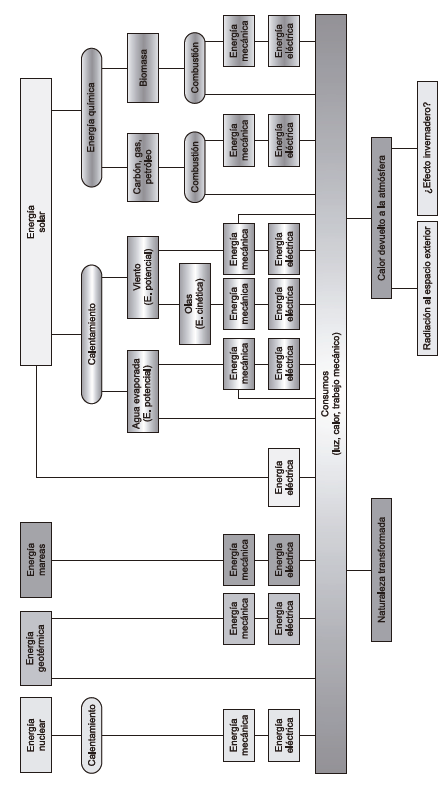
\includegraphics[width=0.45\linewidth, angle=-90]{img/Tranformaciones_energeticas.png}
        \caption{Transformaciones energéticas}
        %\label{fig:enter-label}
    \end{figure}
\end{frame}

\begin{frame}{Equipos utilizados}
    \begin{figure}
        \centering
        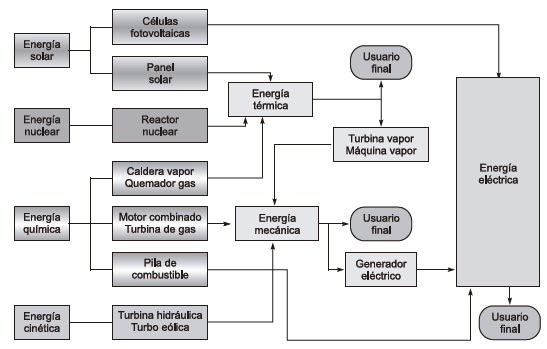
\includegraphics[width=0.7\linewidth]{img/equipos_utilizados.png}
        \caption{Equipos utilizados}
        %\label{fig:enter-label}
    \end{figure}
\end{frame}

\begin{frame}{Definición}
    \begin{itemize}
        \item Conjunto de equipos y procesos para transformar la energía primaria en energía disponible.
        \item Varían en complejidad, desde centrales nucleares y térmicas hasta solares.
    \end{itemize}
\end{frame}

\begin{frame}{¿Qué es una caldera de vapor?}
  \begin{itemize}
    \item Sistema que convierte energía primaria (petróleo, gas, carbón, biomasa, etc.) en vapor de agua a alta temperatura y presión.
    \item Producto adicional: gases calientes de combustión que se liberan a la atmósfera.
  \end{itemize}
  \centering
  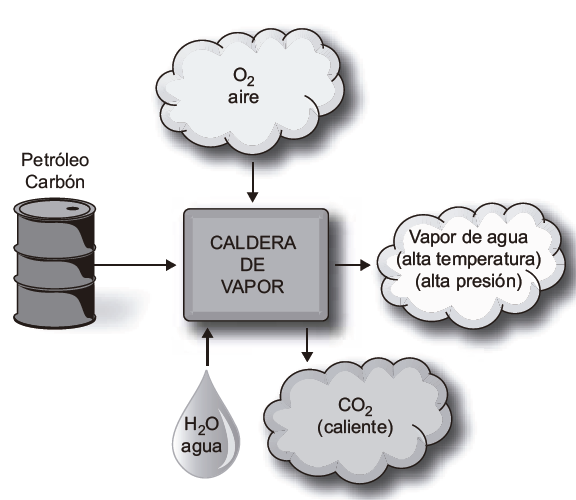
\includegraphics[width=0.4\textwidth]{img/esquema_caldera.png}
\end{frame}

\begin{frame}{Funcionamiento Básico}
  \begin{itemize}
    \item La caldera es un recipiente donde se hierve agua mediante calor de combustión.
    \item En su interior, el agua circula por tubos serpentines adheridos a las paredes internas.
    \item Al calentarse, el agua se transforma en vapor sobrecalentado (700–1000 °C) y a alta presión.
  \end{itemize}
\end{frame}

\begin{frame}{Componentes de una caldera}
  \begin{columns}
    \column{0.5\textwidth}
    \textbf{Principales elementos:}
    \begin{itemize}
      \item Quemadores (principal y piloto)
      \item Ventilador
      \item Parrilla o cinta transportadora (según tipo de combustible)
      \item Entrada de agua fría / Salida de vapor
      \item Paredes refractarias
    \end{itemize}
    \column{0.5\textwidth}
    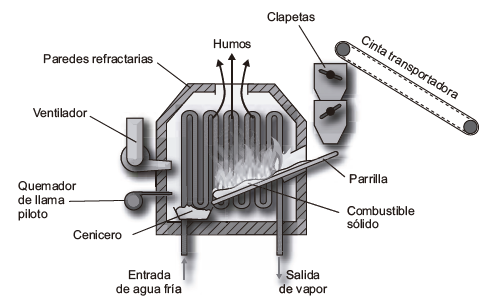
\includegraphics[width=\textwidth]{img/componentes_caldera.png}
  \end{columns}
\end{frame}

\begin{frame}{Tipos de combustibles y quemadores}
  \begin{itemize}
    \item \textbf{Combustibles sólidos:} carbón, biomasa, residuos sólidos.
    \item \textbf{Combustibles líquidos:} petróleo, biodiésel.
    \item \textbf{Combustibles gaseosos:} gas natural, biogás, hidrógeno.
    \item Los quemadores varían en forma y tecnología según el tipo de combustible utilizado.
  \end{itemize}
\end{frame}

\begin{frame}{Sistema de escape y recuperación de calor}
  \begin{itemize}
    \item Los gases de combustión se expulsan por una chimenea.
    \item Parte del calor residual se reutiliza para precalentar el aire de combustión (mejora del rendimiento).
    \item Se incluyen sistemas de recolección de cenizas y precipitadores electrostáticos para capturar partículas.
  \end{itemize}
\end{frame}

\begin{frame}{Motor de Combustión Interna (Alternativo)}
  \begin{itemize}
    \item Convierte energía química de un hidrocarburo (petróleo, gas) en energía mecánica (movimiento de un eje).
    \item Produce además gases calientes de combustión (CO₂, H₂O) liberados a la atmósfera.
  \end{itemize}
  \centering
  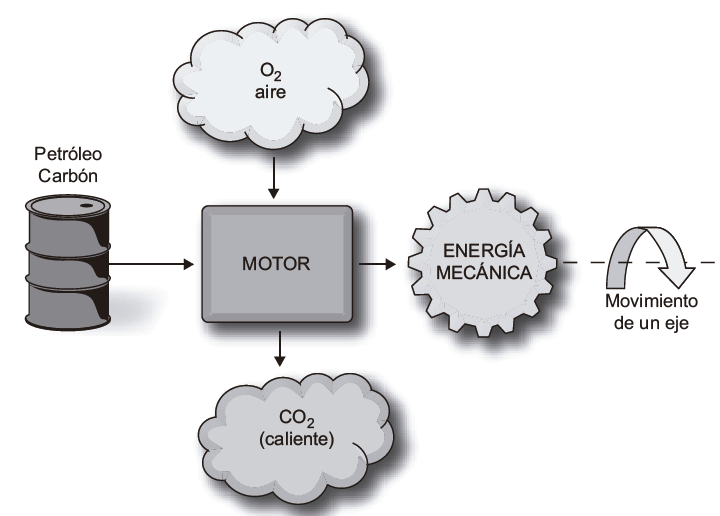
\includegraphics[width=0.5\textwidth]{img/motor_combustion_concepto.png}
\end{frame}

\begin{frame}{Componentes de un Motor Alternativo}
  \begin{itemize}
    \item Cilindro con un pistón en su interior.
    \item Biela que conecta pistón con el cigüeñal.
    \item Cámara de combustión (entre pistón y culata).
    \item Al encender la mezcla aire-combustible, se genera presión que impulsa el pistón.
  \end{itemize}
 % \includegraphics[width=0.55\textwidth]{img/motor_seccion.png}
\end{frame}

\begin{frame}{Sistema de Válvulas y Encendido}
  \begin{itemize}
    \item Válvulas controlan entrada de aire-combustible y salida de gases quemados.
    \item Encendido puede ser:
    \begin{itemize}
      \item Por chispa (bujía): encendido provocado.
      \item Por compresión: autoencendido (motores diésel).
    \end{itemize}
  \end{itemize}
\end{frame}


\begin{frame}{Funcionamiento de un Motor de 4 Tiempos}
  \begin{enumerate}
    \item \textbf{Admisión:} entra aire y combustible (válvula A abierta, E cerrada).
    \item \textbf{Compresión:} se cierran ambas válvulas y el pistón sube.
    \item \textbf{Explosión:} encendido, presión impulsa el pistón hacia abajo.
    \item \textbf{Escape:} se abre válvula E y salen los gases quemados.
  \end{enumerate}
  \centering
  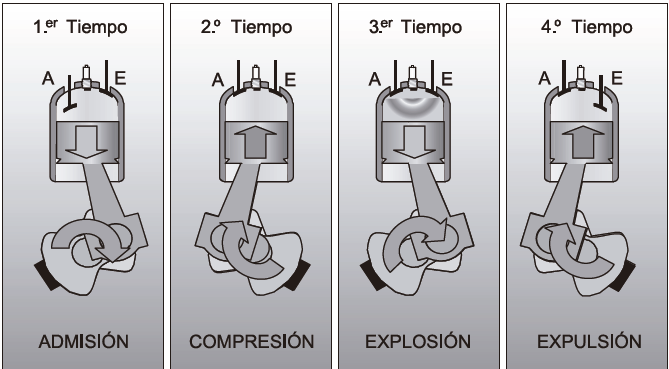
\includegraphics[width=0.6\textwidth]{img/motor_4_tiempos.png}
\end{frame}


\begin{frame}{Características del Motor de 4 Tiempos}
  \begin{itemize}
    \item Realiza una carrera útil cada dos vueltas del cigüeñal.
    \item Funcionamiento irregular: solo 1 de cada 4 tiempos genera trabajo útil.
    \item Necesita volante de inercia para estabilizar el movimiento.
  \end{itemize}
\end{frame}

\begin{frame}{Funcionamiento de un Motor de 2 Tiempos}
  \begin{itemize}
    \item \textbf{1. Compresión:} el pistón sube, comprime mezcla; entra mezcla al cárter.
    \item \textbf{2. Explosión y escape:} explosión impulsa el pistón hacia abajo, salen gases y entra mezcla nueva.
  \end{itemize}
  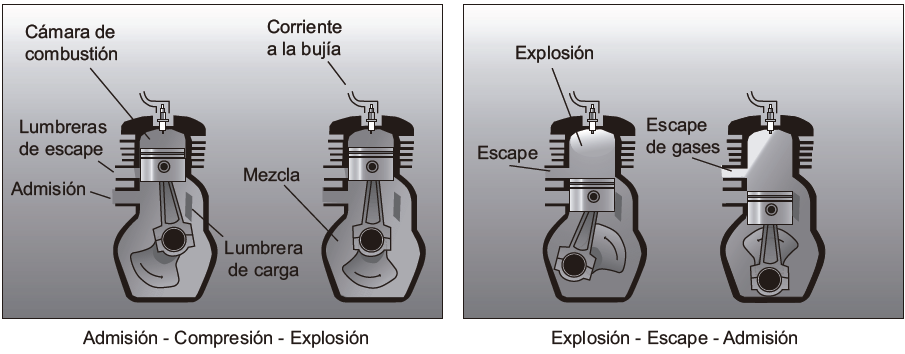
\includegraphics[width=0.75\textwidth]{img/motor_2_tiempos.png}
\end{frame}

\begin{frame}{Comparación y Aplicaciones}
  \begin{itemize}
    \item \textbf{4 tiempos:} mayor eficiencia, menor contaminación, más durabilidad. Usado en autos y maquinaria pesada.
    \item \textbf{2 tiempos:} más potencia por peso, menos piezas, mayor desgaste. Usado en motos, motosierras, motores marinos ligeros.
  \end{itemize}
\end{frame}


\begin{frame}{Turbina de Vapor}
  \begin{itemize}
    \item Convierte la energía térmica del vapor de agua en energía mecánica rotativa.
    \item El vapor proviene de una caldera a alta presión y temperatura (700–1000 °C).
    \item Se utiliza comúnmente en centrales térmicas, nucleares y ciclos combinados.
  \end{itemize}
  \centering
  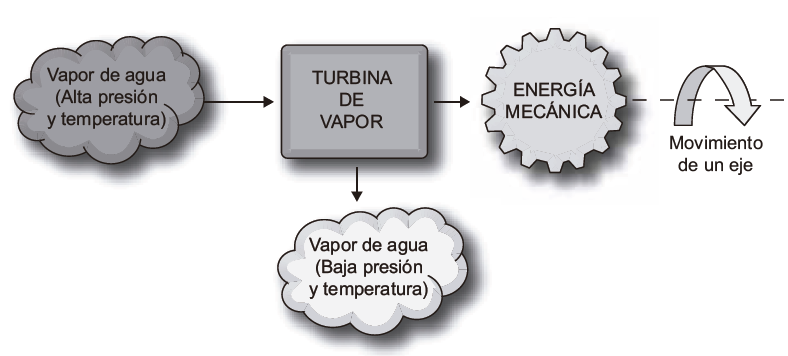
\includegraphics[width=0.7\textwidth]{img/turbina_concepto.png}
\end{frame}


\begin{frame}{Principio de Funcionamiento}
  \begin{itemize}
    \item El vapor a alta presión se acelera en toberas formando un chorro de vapor.
    \item Este chorro impacta los álabes de la turbina, generando giro del eje.
    \item El objetivo es transferir la máxima energía posible al eje mecánico.
  \end{itemize}
  \centering
  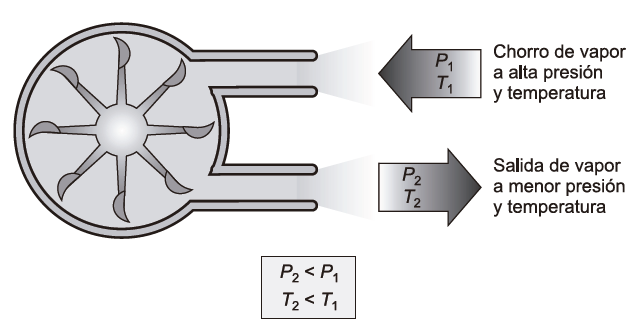
\includegraphics[width=0.7\textwidth]{img/turbina_funcionamiento.png}
\end{frame}

\begin{frame}{Optimización del Rendimiento}
  \begin{itemize}
    \item Para maximizar la eficiencia, el vapor debe entregar la mayor cantidad de energía posible al eje de la turbina.
    \item Esto se logra manteniendo una alta presión y temperatura a la entrada (\(P_{1e}, T_{1e}\)) y reduciendo al máximo estos valores a la salida (\(P_{3s}, T_{3s}\)).
    \item Cuanto mayor sea el salto de presión y temperatura (\(P_{1e} > P_{3s}\), \(T_{1e} > T_{3s}\)), mayor será el aprovechamiento energético.
    \item Es fundamental minimizar las pérdidas por energía cinética remanente en el vapor de escape.
  \end{itemize}
\end{frame}


\begin{frame}{Turbina de Vapor Multietapa}
  \begin{itemize}
    \item Para mejorar la eficiencia, se usan varias etapas (alta, media y baja presión).
    \item Todas las etapas están conectadas al mismo eje rotatorio.
    \item Cada etapa tiene álabes adaptados a su nivel de presión.
  \end{itemize}
  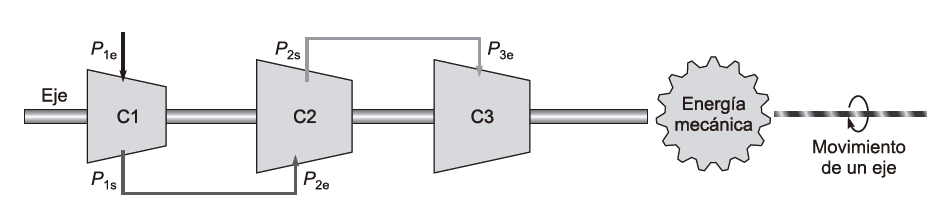
\includegraphics[width=\textwidth]{img/turbina_multietapa.png}
\end{frame}


\begin{frame}{Presiones en Turbina Multietapa}
  \begin{itemize}
    \item \textbf{Etapa de alta presión:} el vapor entra a presión \(P_{1e}\) y sale a \(P_{1s}\). Se emplean álabes pequeños y numerosos.
    \item \textbf{Etapa de media presión:} el vapor entra a \(P_{2e} \approx P_{1s}\) y sale a \(P_{2s}\). Los álabes son de tamaño intermedio.
    \item \textbf{Etapa de baja presión:} el vapor entra a \(P_{3e} \approx P_{2s}\) y sale a \(P_{3s}\), la presión más baja del ciclo. Los álabes son grandes y de diseño aerodinámico.
  \end{itemize}
\end{frame}


\begin{frame}{Tipos de Flujo en Turbinas}
  \begin{itemize}
    \item \textbf{Flujo axial:} el vapor se desplaza paralelo al eje de rotación. \\
    Uso común en grandes turbinas de generación eléctrica.
    \item \textbf{Flujo radial:} el vapor se desplaza desde el centro hacia la periferia. \\
    Diseño más compacto, pero generalmente menos eficiente que el axial.
  \end{itemize}
\end{frame}



\begin{frame}{Rotor de una Turbina de Vapor}
  \begin{itemize}
    \item Componente clave donde se montan los álabes.
    \item Debe resistir altas temperaturas y esfuerzos centrífugos.
    \item Fabricado en aleaciones especiales resistentes a la corrosión térmica.
  \end{itemize}
  \begin{center}
    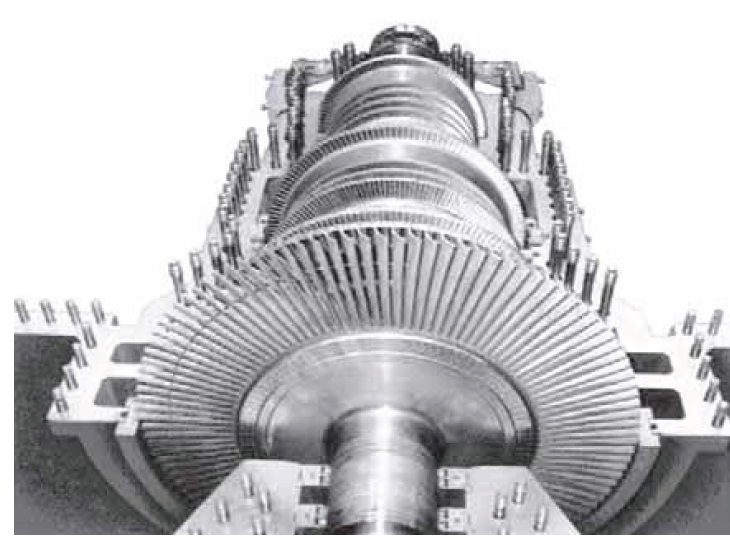
\includegraphics[width=0.5\textwidth]{img/rotor_turbina.png}
  \end{center}
\end{frame}


\begin{frame}{Aplicaciones en 2025}
  \begin{itemize}
    \item Generación de energía en ciclos Rankine y ciclos combinados.
    \item Uso en centrales nucleares, geotérmicas e industriales.
    \item Con turbinas de alta eficiencia, se logran rendimientos térmicos superiores al 42\,\%.
  \end{itemize}
\end{frame}


\begin{frame}{¿Qué es un Intercambiador de Calor?}
  \begin{itemize}
    \item Es un dispositivo que permite transferir energía térmica entre dos fluidos sin que se mezclen.
    \item Se utiliza ampliamente en procesos industriales, centrales térmicas, sistemas HVAC y refrigeración.
    \item Mejora la eficiencia energética al recuperar o disipar calor.
  \end{itemize}
  \centering
  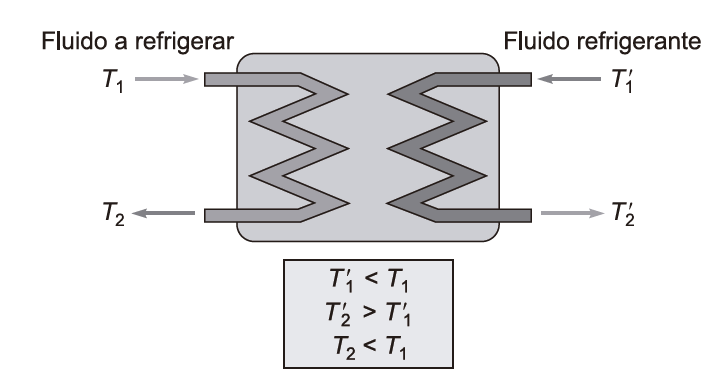
\includegraphics[width=0.6\textwidth]{img/intercambiador_concepto.png}
\end{frame}

\begin{frame}{Estructura Básica}
  \begin{itemize}
    \item Generalmente formado por placas o tubos contiguos.
    \item Los fluidos circulan separados, en configuraciones de flujo paralelo o contracorriente.
    \item Se favorece la transferencia de calor mediante gran área superficial y conducción térmica eficiente.
  \end{itemize}
  \centering
  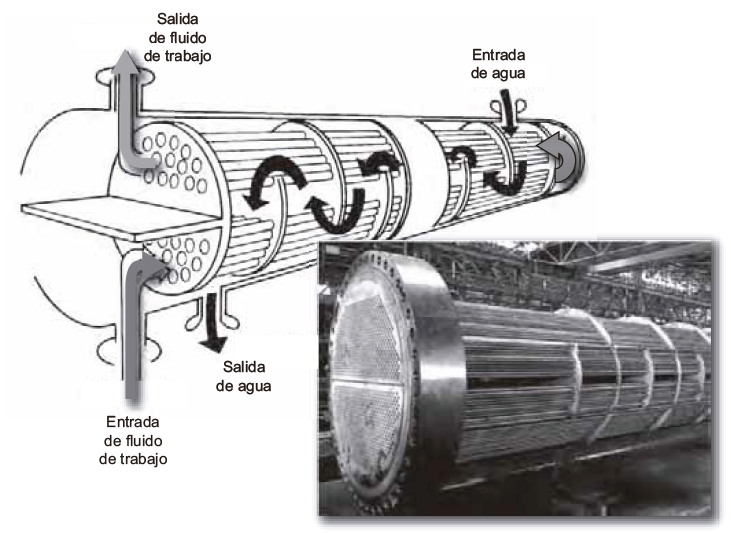
\includegraphics[width=0.45\textwidth]{img/intercambiador_esquema.png}
\end{frame}


\begin{frame}{Tipos de Intercambiadores según los Fluidos}
  \begin{itemize}
    \item \textbf{Gas-gas:} utilizado en turbinas de gas, calderas, recuperadores de calor de chimeneas.
    \item \textbf{Líquido-líquido:} común en industrias químicas, alimentarias y de procesos térmicos.
    \item \textbf{Gas-líquido:} empleado en condensadores, evaporadores y torres de enfriamiento.
  \end{itemize}
\end{frame}


\begin{frame}{Condensadores: Intercambiadores Especiales}
  \begin{itemize}
    \item Cuando el fluido caliente entra en estado gaseoso y sale en estado líquido, el intercambiador actúa como un \textbf{condensador}.
    \item Muy usado en turbinas de vapor, sistemas de refrigeración, aire acondicionado y ciclos Rankine.
    \item Ejemplo en 2025: condensadores con microcanales para mejorar la transferencia de calor en centrales solares térmicas.
  \end{itemize}
\end{frame}

\begin{frame}{¿Qué es una Turbina de Gas?}
  \begin{itemize}
    \item Convierte la energía química del combustible (gas, petróleo) en energía mecánica mediante gases de combustión.
    \item Similar a la turbina de vapor, pero el fluido de trabajo es una mezcla de gases calientes generados en una cámara de combustión.
    \item Utilizada ampliamente en generación eléctrica, aviación y ciclos combinados.
  \end{itemize}
  \centering
  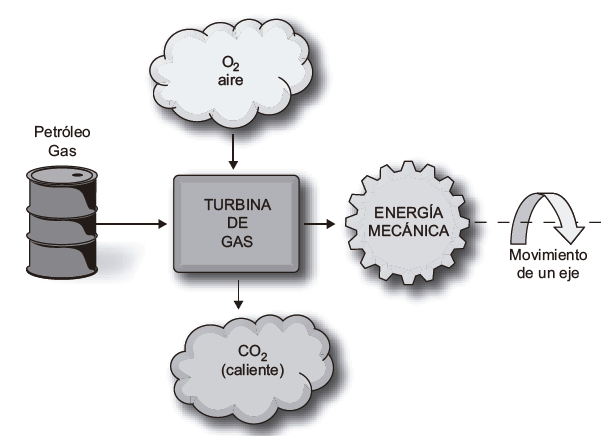
\includegraphics[width=0.4\textwidth]{img/turbina_gas_concepto.png}
\end{frame}


\begin{frame}{Componentes de una Turbina de Gas}
  \begin{itemize}
    \item \textbf{Compresor:} comprime el aire antes de entrar a la cámara de combustión.
    \item \textbf{Cámara de combustión:} se mezcla aire comprimido con combustible y se inflama.
    \item \textbf{Turbina:} convierte la energía de los gases calientes en energía mecánica (rotación del eje).
  \end{itemize}
  \centering
  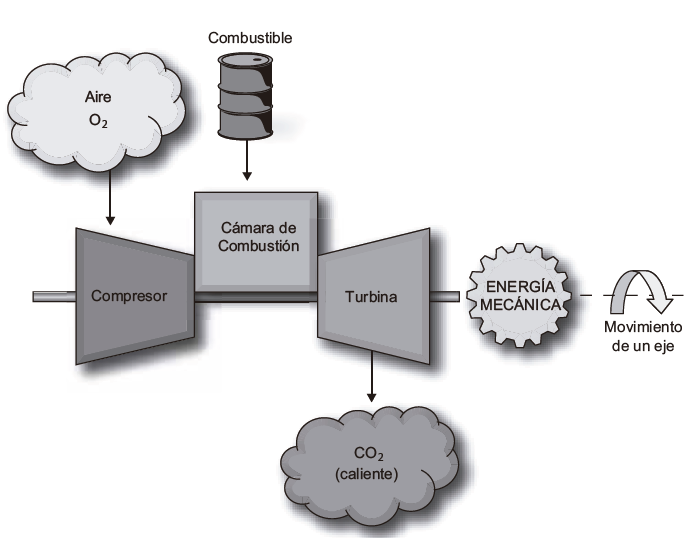
\includegraphics[width=0.4\textwidth]{img/componentes_turbina_gas.png}
\end{frame}

\begin{frame}{Funcionamiento y Eficiencia}
  \begin{itemize}
    \item El eje del compresor y la turbina están acoplados: cerca del 50\% de la energía se utiliza en el propio compresor.
    \item La eficiencia global de una turbina de gas en ciclo abierto es del 30--40\%.
    \item La temperatura de entrada a la turbina puede alcanzar los 1200\textdegree C; la de salida, unos 500\textdegree C.
  \end{itemize}
\end{frame}


\begin{frame}{Etapas de Compresor y Turbina}
  \begin{itemize}
    \item Para mejorar el rendimiento, el compresor cuenta con 10 a 20 etapas.
    \item La turbina suele tener entre 3 y 4 etapas para expandir eficientemente los gases calientes.
    \item Esto permite aumentar la presión y temperatura progresivamente, optimizando la conversión energética.
  \end{itemize}
  \centering
  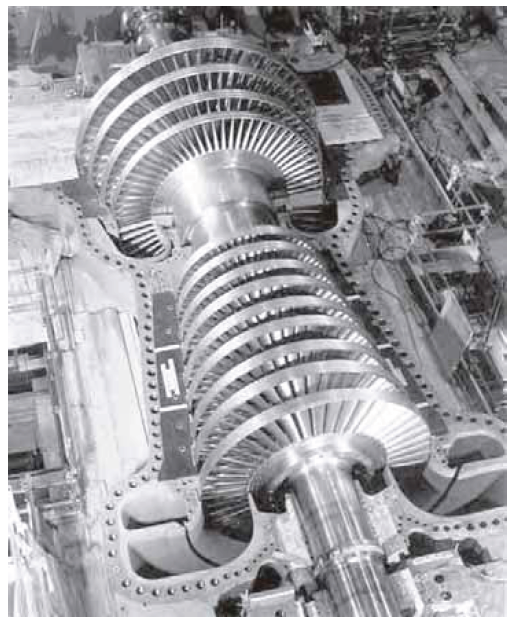
\includegraphics[width=0.3\textwidth]{img/rotor_turbina_gas.png}
\end{frame}


\begin{frame}{Ciclo Abierto vs Ciclo Cerrado}
  \begin{itemize}
    \item \textbf{Ciclo abierto:} el aire entra desde la atmósfera al compresor y los gases de escape se liberan directamente.
    \item \textbf{Ciclo cerrado:} el fluido de trabajo (gas o líquido presurizado) circula en circuito cerrado, calentado mediante intercambiadores externos.
    \item El ciclo cerrado es más eficiente térmicamente y permite mayor control del entorno de operación.
  \end{itemize}
  \centering
  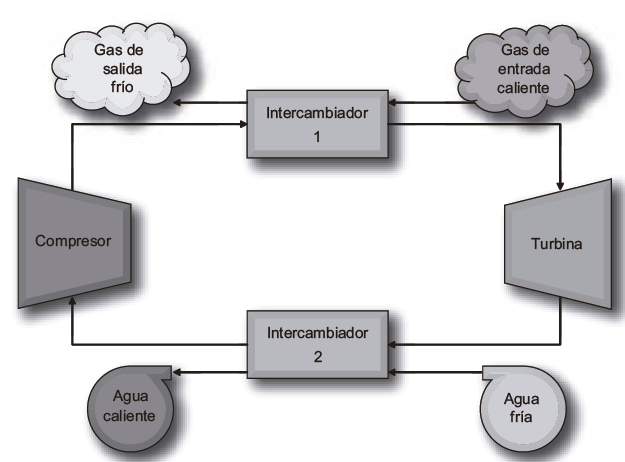
\includegraphics[width=0.4\textwidth]{img/ciclo_cerrado_turbina_gas.png}
\end{frame}


\begin{frame}{Aplicaciones en 2025}
  \begin{itemize}
    \item Generación eléctrica en plantas de ciclo combinado (con turbina de vapor acoplada).
    \item Propulsión de aeronaves (motores a reacción y turbohélices).
    \item Generación distribuida y respaldo en redes eléctricas inteligentes.
    \item Operación en ambientes extremos, como plataformas offshore o unidades militares móviles.
  \end{itemize}
\end{frame}

\begin{frame}{¿Qué es una Turbina Hidráulica?}
  \begin{itemize}
    \item Convierte la energía cinética del agua en energía mecánica rotativa.
    \item El agua proviene de un embalse o río y se canaliza para impactar los álabes de la turbina.
    \item El principio de funcionamiento es similar al de una turbina de vapor, pero utilizando agua como fluido de trabajo.
  \end{itemize}
  \centering
  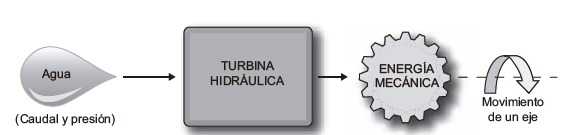
\includegraphics[width=\textwidth]{img/turbina_hidraulica_concepto.png}
\end{frame}

\begin{frame}{Origen de la Energía del Agua}
  \begin{itemize}
    \item El agua posee energía potencial debido a la diferencia de altura entre dos puntos (salto hidráulico).
    \item Al fluir desde un embalse superior hacia uno inferior, esta energía se convierte en cinética.
    \item La velocidad del chorro de agua impacta los álabes de la turbina, provocando su rotación.
  \end{itemize}
\end{frame}

\begin{frame}{Tipos de Turbinas según Altura y Caudal}
  \begin{itemize}
    \item \textbf{Altura elevada, bajo caudal:} turbina Pelton (tipo de acción).
    \item \textbf{Altura media, caudal medio:} turbina Francis (tipo mixto).
    \item \textbf{Baja altura, alto caudal:} turbina Kaplan (tipo de reacción).
  \end{itemize}
 % \includegraphics[width=0.6\textwidth]{tipos_turbinas_hidraulicas.png}
\end{frame}

\begin{frame}{Clasificación Funcional de Turbinas Hidráulicas}
  \begin{itemize}
    \item \textbf{Turbinas de acción:} utilizan solo la velocidad del chorro de agua (e.g., Pelton).
    \item \textbf{Turbinas de reacción:} aprovechan velocidad y presión del flujo (e.g., Francis, Kaplan).
    \item La elección depende de condiciones hidráulicas locales: altura neta, caudal disponible y uso requerido.
  \end{itemize}
\end{frame}

\begin{frame}{Aplicaciones en 2025}
  \begin{itemize}
    \item Generación hidroeléctrica en centrales de gran, mediana y pequeña escala.
    \item Uso combinado en microturbinas con sistemas de almacenamiento energético.
    \item Integración en soluciones de energía distribuida en zonas rurales y remotas.
    \item Desarrollos modernos incluyen turbinas reversibles en plantas de bombeo-turbina.
  \end{itemize}
\end{frame}


\begin{frame}{¿Qué es una Turbina Eólica?}
  \begin{itemize}
    \item Dispositivo que convierte la energía cinética del viento en energía mecánica rotativa.
    \item El aire en movimiento impacta las palas del rotor, haciendo girar el eje (buje).
    \item Similar en concepto a otras turbinas, pero con características aerodinámicas específicas.
  \end{itemize}
  \centering
  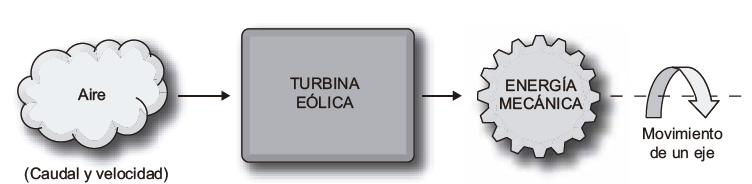
\includegraphics[width=0.65\textwidth]{img/turbina_eolica_concepto.png}
\end{frame}



\begin{frame}{Estructura de una Turbina Eólica}
  \begin{itemize}
    \item \textbf{Rotor:} conjunto de palas y buje que capta la energía del viento.
    \item \textbf{Buje:} eje central que transmite el giro al generador.
    \item \textbf{Torre:} soporte estructural que eleva el rotor a mayor altura donde el viento es más constante.
    \item \textbf{Generador:} transforma energía mecánica en eléctrica.
  \end{itemize}
\end{frame}

\begin{frame}{Tipos de Rotores en Turbinas Eólicas}
  \begin{itemize}
    \item \textbf{Multipala (rotor lento):} 6 a 24 palas, usado en bombeo y aplicaciones rurales.
    \item \textbf{Tipo hélice (rotor rápido):} 1, 2 o 3 palas; usado en generación eléctrica.
    \item La mayoría de los aerogeneradores modernos son tripalas por eficiencia y estabilidad.
  \end{itemize}
\end{frame}


\begin{frame}{Potencia Captada y Tamaño del Rotor}
  \begin{itemize}
    \item La potencia extraída del viento es proporcional al cubo de su velocidad: \( P \propto v^3 \).
    \item También depende del área barrida por el rotor: \( A = \frac{\pi D^2}{4} \), donde \( D \) es el diámetro del rotor.
    \item En 2025 existen rotores de más de 120 m de diámetro que alcanzan potencias superiores a 10 MW.
  \end{itemize}
\end{frame}



\begin{frame}{Aplicaciones en 2025}
  \begin{itemize}
    \item Generación eléctrica a gran escala en parques eólicos onshore y offshore.
    \item Integración en microredes y sistemas híbridos con almacenamiento.
    \item Turbinas verticales y urbanas para entornos residenciales o comerciales.
    \item Desarrollo de aerogeneradores flotantes en alta mar para aprovechar vientos marinos constantes.
  \end{itemize}
\end{frame}

\begin{frame}{¿Qué es una Pila de Combustible?}
  \begin{itemize}
    \item Dispositivo electroquímico que convierte directamente la energía química del hidrógeno o gases combustibles en electricidad.
    \item No posee partes móviles; es silenciosa, eficiente y sin emisiones contaminantes locales.
    \item Produce electricidad (corriente continua), calor y agua como subproducto.
  \end{itemize}
  \centering
  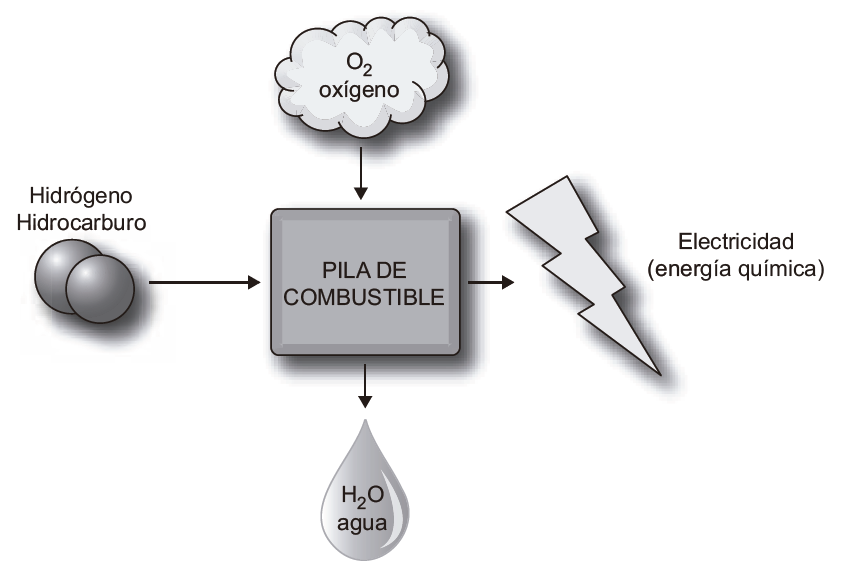
\includegraphics[width=0.5\textwidth]{img/pila_combustible_concepto.png}
\end{frame}

\begin{frame}{Estructura de una Celda de Combustible}
  \begin{itemize}
    \item Compuesta por:
    \begin{itemize}
      \item Ánodo y cátodo
      \item Electrolito y catalizador
      \item Membrana de intercambio protónico (PEM)
      \item Placas colectoras de corriente
    \end{itemize}
    \item Las celdas se conectan en serie para formar una pila completa.
  \end{itemize}
  \centering
  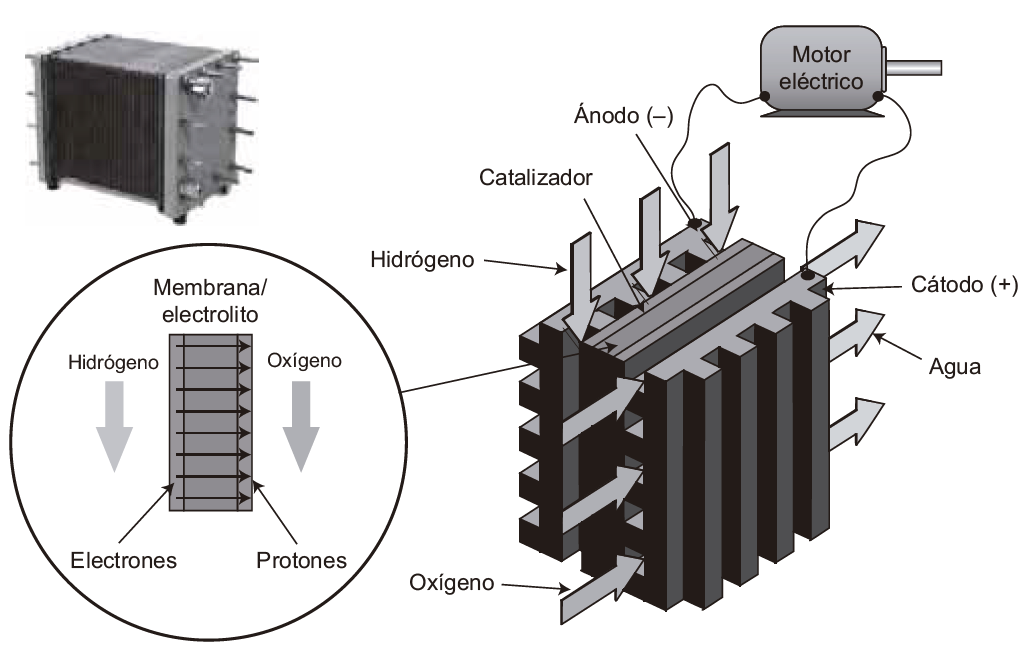
\includegraphics[width=0.4\textwidth]{img/celda_combustible_esquema.png}
\end{frame}

\begin{frame}{Reacciones en la Celda de Combustible}
  \begin{itemize}
    \item \textbf{Ánodo:} \(2\text{H}_2 \rightarrow 4\text{H}^+ + 4e^-\)
    \item \textbf{Cátodo:} \(\text{O}_2 + 4\text{H}^+ + 4e^- \rightarrow 2\text{H}_2\text{O}\)
    \item \textbf{Reacción global:} \(2\text{H}_2 + \text{O}_2 \rightarrow 2\text{H}_2\text{O}\)
    \item Genera electricidad y calor de forma eficiente y continua mientras se suministren los reactivos.
  \end{itemize}
\end{frame}

\begin{frame}{Tipos de Pilas de Combustible (2025)}
  \begin{itemize}
    \item \textbf{PEFC (polímero):} 80\,°C – aplicaciones móviles y portátiles.
    \item \textbf{AFC (alcalina):} 100\,°C – aplicaciones espaciales y militares.
    \item \textbf{PAFC (ácido fosfórico):} 200\,°C – cogeneración en edificios.
    \item \textbf{MCFC (carbonatos fundidos):} 650\,°C – plantas estacionarias.
    \item \textbf{SOFC (óxidos sólidos):} 950\,°C – generación eléctrica en megavatios.
  \end{itemize}
\end{frame}

\begin{frame}{Eficiencia y Aplicaciones en 2025}
  \begin{itemize}
    \item Eficiencia real: 45--60\%, superior a motores térmicos convencionales.
    \item Empleadas en:
    \begin{itemize}
      \item Transporte (vehículos eléctricos de hidrógeno)
      \item Generación distribuida y respaldo de emergencia
      \item Sistemas portátiles y militares
    \end{itemize}
    \item Desarrollos actuales permiten integración con electrolizadores y energías renovables.
  \end{itemize}
\end{frame}


\begin{frame}{Generador y Motor Eléctrico}
  \begin{itemize}
    \item \textbf{Generador:} convierte energía mecánica (giro de un eje) en energía eléctrica.
    \item \textbf{Motor:} transforma energía eléctrica en energía mecánica (movimiento rotatorio).
    \item Ambos son dispositivos electromagnéticos basados en la interacción entre campos magnéticos y conductores.
  \end{itemize}
  \centering
  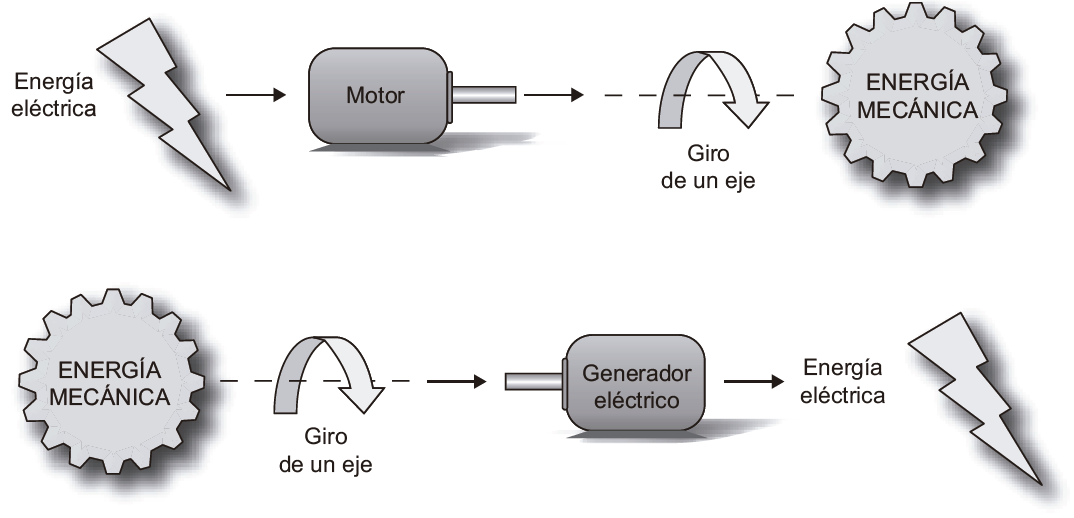
\includegraphics[width=0.6\textwidth]{img/generador_motor_concepto.png}
\end{frame}

\begin{frame}{Principio del Generador Eléctrico}
  \begin{itemize}
    \item Al mover un conductor dentro de un campo magnético, se genera una \textbf{fuerza electromotriz} (FEM).
    \item Esto induce una corriente eléctrica en el conductor.
    \item La dirección de la corriente depende del sentido del movimiento y del campo, y se determina mediante la \textbf{regla de la mano izquierda}.
  \end{itemize}
  \centering
  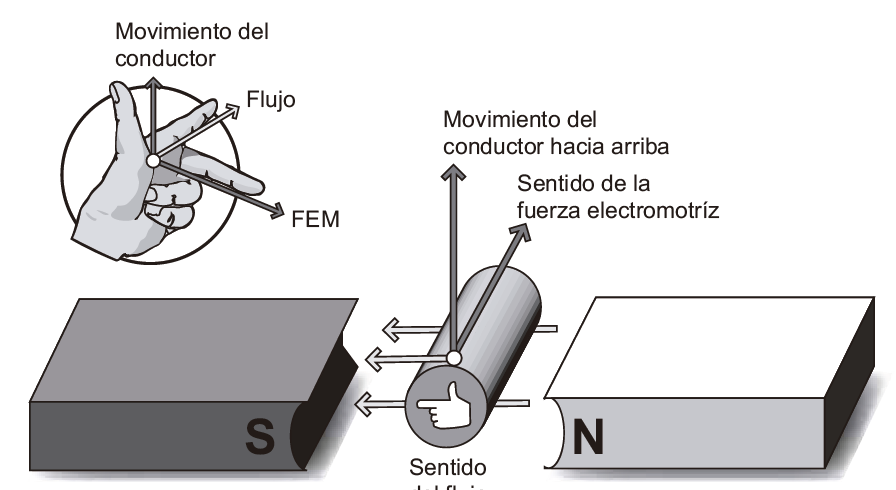
\includegraphics[width=0.5\textwidth]{img/regla_mano_izquierda.png}
\end{frame}

\begin{frame}{Generador Eléctrico Elemental}
  \begin{itemize}
    \item Consiste en una espira giratoria dentro de un campo magnético entre dos polos (N y S).
    \item La espira está conectada a anillos rozantes y escobillas que permiten transferir la corriente al circuito externo.
    \item El giro de la espira produce una corriente alterna senoidal.
  \end{itemize}
  \centering
  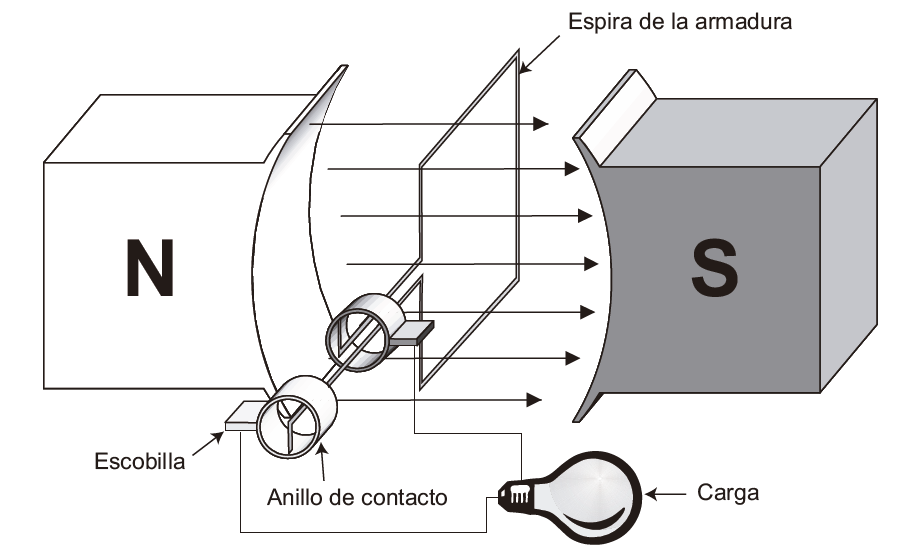
\includegraphics[width=0.5\textwidth]{img/generador_elemental.png}
\end{frame}

\begin{frame}{Corriente Alterna Generada}
  \begin{itemize}
    \item El voltaje inducido varía de forma senoidal debido a la rotación de la espira en el campo magnético.
    \item En una vuelta completa: 
    \begin{itemize}
      \item Se genera un máximo positivo.
      \item Luego, vuelve a cero y alcanza un valor negativo.
      \item Finalmente, regresa a cero.
    \end{itemize}
    \item Resultado: una señal de corriente alterna (CA), típica en sistemas eléctricos de potencia.
  \end{itemize}
\end{frame}

\begin{frame}{Principio del Motor Eléctrico}
  \begin{itemize}
    \item Funciona de forma inversa al generador.
    \item Una corriente eléctrica que pasa por una espira en un campo magnético genera una \textbf{fuerza mecánica}.
    \item Esta fuerza produce el giro del eje, convirtiendo electricidad en movimiento.
    \item Ampliamente utilizado en electrodomésticos, vehículos eléctricos, robótica e industria.
  \end{itemize}
\end{frame}

\begin{frame}{Aplicaciones Modernas en 2025}
  \begin{itemize}
    \item \textbf{Generadores:} turbinas eólicas, hidroeléctricas, grupos electrógenos y plantas de energía renovable.
    \item \textbf{Motores:} vehículos eléctricos, automatización industrial, robótica, bombas, ventiladores.
    \item Integración con energías renovables, redes inteligentes y sistemas de almacenamiento.
  \end{itemize}
\end{frame}

\begin{frame}{¿Qué es un Transformador Eléctrico?}
  \begin{itemize}
    \item Dispositivo electromagnético que modifica los valores de tensión e intensidad de una corriente alterna sin cambiar su frecuencia.
    \item Eleva o reduce la tensión, manteniendo constante la potencia (idealmente).
    \item Fundamental en los sistemas de transmisión y distribución eléctrica.
  \end{itemize}
  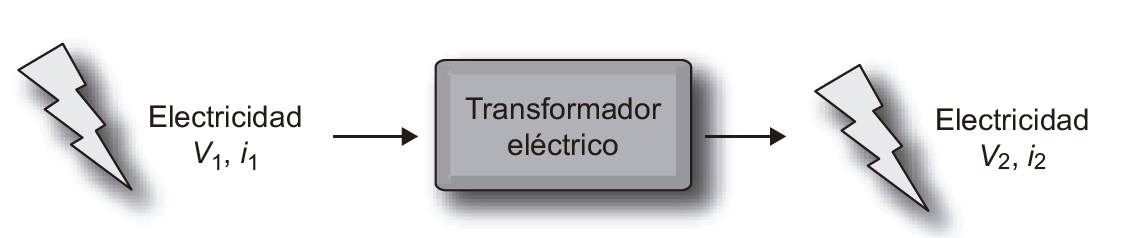
\includegraphics[width=0.6\textwidth]{img/transformador_concepto.png}
\end{frame}

\begin{frame}{Principio de Funcionamiento}
  \begin{itemize}
    \item Basado en la inducción electromagnética: un campo magnético variable genera corriente en un conductor cercano.
    \item La corriente alterna en la bobina primaria genera un campo magnético oscilante.
    \item Este campo induce corriente alterna en la bobina secundaria.
  \end{itemize}
%  \includegraphics[width=0.5\textwidth]{campo_inducido_transformador.png}
\end{frame}

\begin{frame}{Relación de Transformación}
  \begin{itemize}
    \item La relación de tensiones depende del número de espiras:
    \[
      \frac{V_2}{V_1} = \frac{N_2}{N_1}
    \]
    \item Si \(N_2 > N_1\): transformador elevador de tensión.
    \item Si \(N_2 < N_1\): transformador reductor de tensión.
  \end{itemize}
\end{frame}

\begin{frame}{Conservación de Potencia}
  \begin{itemize}
    \item En condiciones ideales: \( V_1 \cdot I_1 = V_2 \cdot I_2 \)
    \item Si se eleva la tensión, disminuye la intensidad, y viceversa.
    \item Esto permite:
    \begin{itemize}
      \item Transmitir energía con cables más delgados.
      \item Reducir pérdidas por efecto Joule, que son proporcionales a \( I^2 \cdot R \).
    \end{itemize}
  \end{itemize}
\end{frame}

\begin{frame}{Ventajas en la Transmisión de Energía}
  \begin{itemize}
    \item Disminuir la intensidad en la red de alta tensión permite:
    \begin{itemize}
      \item Reducir el calibre de los conductores.
      \item Disminuir las pérdidas térmicas (hasta 4 veces si se duplica la tensión).
    \end{itemize}
    \item En 2025, se utilizan transformadores de hasta 800 kV en líneas de transmisión HVDC.
    \item Transformadores inteligentes permiten monitoreo, control remoto y eficiencia mejorada.
  \end{itemize}
\end{frame}

\begin{frame}{Ejemplo de Transformador Eléctrico}
  \begin{center}
    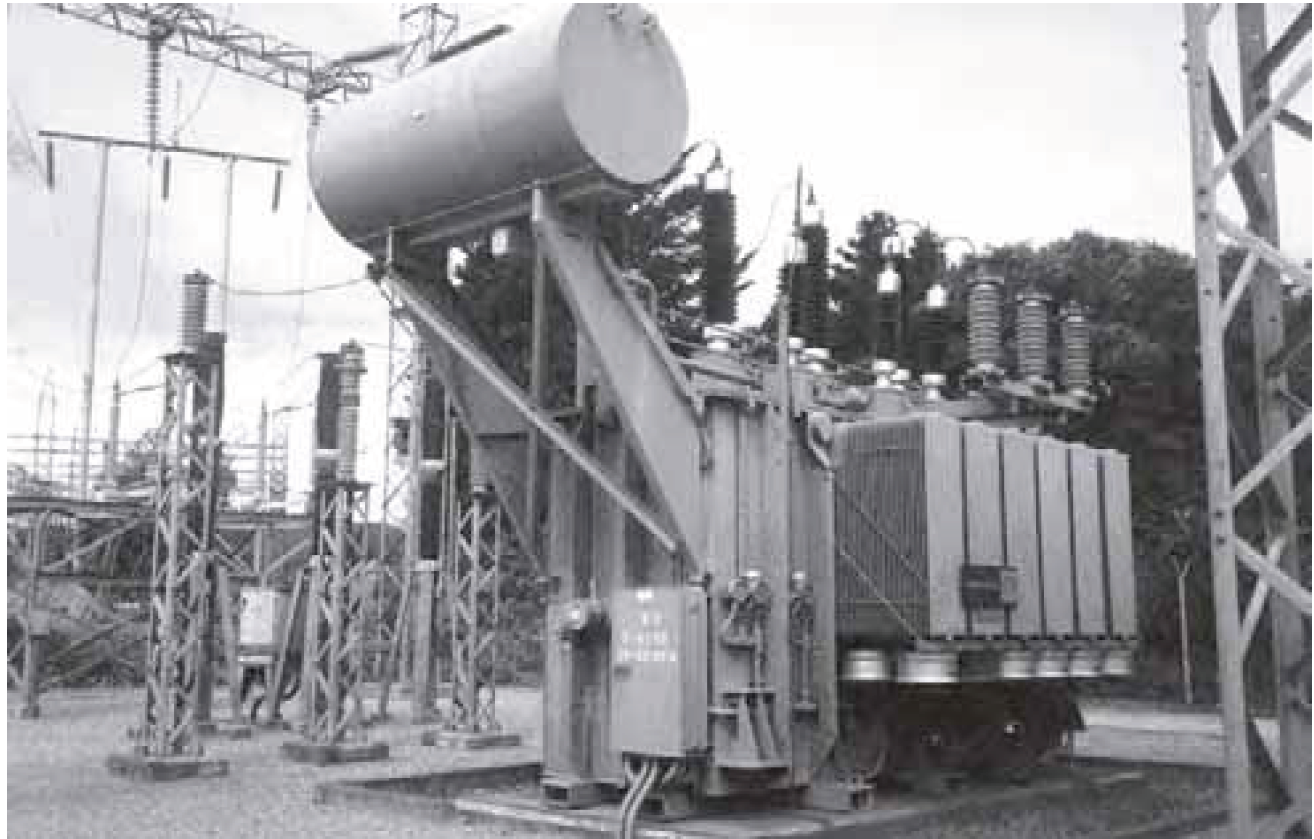
\includegraphics[width=0.65\textwidth]{img/transformador_foto.png}
  \end{center}
  \begin{itemize}
    \item Imagen de un transformador de potencia utilizado en subestaciones de media y alta tensión.
  \end{itemize}
\end{frame}

\begin{frame}{¿Qué son los Vectores Energéticos?}
  \begin{itemize}
    \item Son los medios por los cuales la energía se transporta desde el punto de producción hasta el punto de consumo.
    \item Pueden ser físicos (electricidad, combustibles) o mecánicos (árboles de transmisión, poleas, neumáticos).
    \item Son fundamentales para la funcionalidad de cualquier sistema energético moderno.
  \end{itemize}
\end{frame}

\begin{frame}{Tipos de Vectores Energéticos}
  \begin{itemize}
    \item \textbf{Electricidad:} líneas de alta, media y baja tensión, subestaciones, transformadores.
    \item \textbf{Combustibles sólidos:} carbón, biomasa, transportados por camiones o cintas.
    \item \textbf{Combustibles líquidos:} petróleo y derivados, transportados por oleoductos, buques o cisternas.
    \item \textbf{Combustibles gaseosos:} gas natural, biogás, hidrógeno. Transportados por gaseoductos o en estado licuado.
    \item \textbf{Mecánicos:} transmisiones por ejes, poleas, sistemas hidráulicos y neumáticos.
  \end{itemize}
\end{frame}

\begin{frame}{Transporte de Electricidad}
  \begin{itemize}
    \item Requiere transformación de la tensión:
    \begin{itemize}
      \item Elevación de tensión para transporte a larga distancia.
      \item Reducción de tensión para consumo doméstico o industrial.
    \end{itemize}
    \item Incluye: subestaciones, transformadores, líneas aéreas o subterráneas, y sistemas de protección y control.
    \item En 2025, se usan redes inteligentes (smart grids) y líneas HVDC para mejorar eficiencia y control.
  \end{itemize}
\end{frame}

\begin{frame}{Transporte de Combustibles Líquidos y Gaseosos}
  \begin{itemize}
    \item \textbf{Líquidos:} se transportan mediante oleoductos, buques petroleros, cisternas y tuberías.
    \item \textbf{Gaseosos:} gas natural, hidrógeno, biogás.
    \begin{itemize}
      \item Gaseoductos para transporte a presión.
      \item Depósitos criogénicos si se transportan en estado líquido.
    \end{itemize}
    \item Implican sistemas de almacenamiento primario, secundario y distribución final.
  \end{itemize}
\end{frame}

\begin{frame}{El Hidrógeno como Vector Energético}
  \begin{itemize}
    \item No se encuentra libre en la naturaleza: debe ser producido.
    \item Alta densidad energética y residuo ambiental nulo (solo agua).
    \item Puede almacenarse en forma gaseosa, líquida o absorbido en materiales como zeolitas.
    \item Se transporta por gaseoductos o en tanques presurizados.
    \item Clave para descarbonizar sectores como el transporte pesado e industrial.
  \end{itemize}
\end{frame}

\begin{frame}{Producción de Hidrógeno en 2025}
  \begin{itemize}
    \item \textbf{Steam reforming:} a partir de gas natural. Predominante pero emite CO\textsubscript{2}.
    \item \textbf{Electrólisis del agua:} separación de H\textsubscript{2} y O\textsubscript{2} mediante corriente eléctrica.
    \begin{itemize}
      \item Si la electricidad proviene de renovables, el hidrógeno es totalmente limpio.
    \end{itemize}
    \item \textbf{Otros métodos en desarrollo:}
    \begin{itemize}
      \item Termoquímicos (alta temperatura).
      \item Fotolíticos (uso de luz solar).
    \end{itemize}
  \end{itemize}
\end{frame}

\begin{frame}{Hidrógeno Renovable: Energía Limpia y Almacenamiento}
  \begin{itemize}
    \item Permite transformar la energía solar y eólica en combustible limpio.
    \item Puede almacenarse y usarse posteriormente para:
    \begin{itemize}
      \item Generación eléctrica (pila de combustible).
      \item Combustible para transporte.
      \item Uso industrial (siderurgia, química, fertilizantes).
    \end{itemize}
    \item Representa una solución clave para el almacenamiento energético estacional.
  \end{itemize}
\end{frame}




\begin{frame}{Tipos de Centrales Energéticas}
    \begin{itemize}
        \item Centrales térmicas: queman carbón, petróleo o gas.
        \item Centrales nucleares: utilizan reacciones nucleares para generar calor.
        \item Centrales solares: convierten directamente la luz solar en electricidad.
    \end{itemize}
\end{frame}



\begin{frame}{Componentes de una Central Térmica}
    \begin{columns}
        \column{0.5\textwidth}
        \begin{itemize}
            \item \textbf{Caldera}: convierte agua en vapor usando combustible.
            \item \textbf{Turbina de vapor}: transforma energía térmica en energía mecánica.
            \item \textbf{Generador eléctrico}: convierte energía mecánica en eléctrica.
            \item \textbf{Intercambiador (condensador)}: enfría el vapor para su reutilización.
            \item \textbf{Transformador}: eleva la tensión de la electricidad generada.
        \end{itemize}
        
        \column{0.5\textwidth}
        \begin{center}
            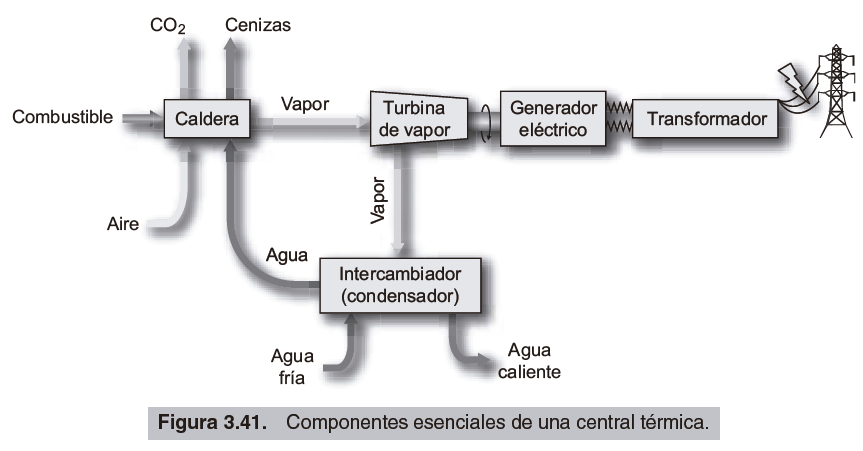
\includegraphics[width=\linewidth]{img/central termica.png} % Imagen referenciada
        \end{center}
    \end{columns}
\end{frame}

\begin{frame}{Proceso de Transformación de Energía}
    \begin{enumerate}
        \item Energía del combustible calienta agua en la caldera, generando vapor.
        \item Vapor a alta presión mueve la turbina de vapor.
        \item Turbina acciona el generador eléctrico para producir electricidad.
        \item El vapor se enfría en un condensador y se recircula.
        \item La electricidad generada es transformada y distribuida.
    \end{enumerate}
\end{frame}

\begin{frame}{Plantas de Ciclo Combinado}
    \begin{columns}
        \column{0.5\textwidth}
        \begin{itemize}
            \item Mejoran el rendimiento de las turbinas de gas al acoplarlas a una turbina de vapor.
            \item Los gases calientes de la turbina de gas calientan agua en un intercambiador gas-agua.
            \item El vapor producido se inyecta en una turbina de vapor.
            \item El rendimiento eléctrico puede alcanzar el 50\%.
        \end{itemize}
        
        \column{0.5\textwidth}
        \centering
        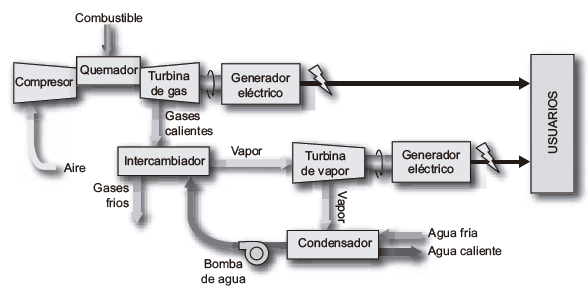
\includegraphics[width=\linewidth]{img/central siclo conbinado.png} % Reemplazar con la ruta correcta de la imagen
    \end{columns}
\end{frame}

    % Diapositiva: Turbina de vapor de contrapresión
\begin{frame}{Turbina de Vapor de Contrapresión}
    \begin{itemize}
        \item Se inyecta agua en la caldera desde el exterior.
        \item El agua se transforma en vapor, que mueve la turbina.
        \item El vapor saliente se usa directamente tras bajar su presión.
        \item El sistema opera en circuito abierto, lo que reduce el rendimiento.
    \end{itemize}
    \begin{center}
        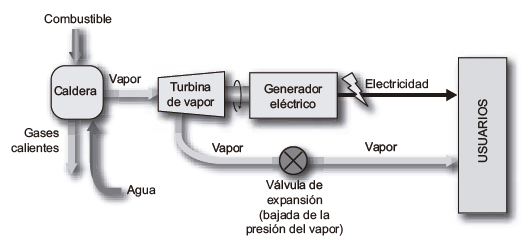
\includegraphics[width=0.7\linewidth]{img/turbina de vapor de contraprestacion.png} % Agregar imagen si se dispone
    \end{center}
\end{frame}

\begin{frame}
    \frametitle{Turbina de Vapor de Condensaci\'on}
    \begin{columns}
        \column{0.5\textwidth}
        \begin{itemize}
            \item En este sistema, parte del vapor se condensa y recircula en la caldera y turbina, y otra parte se emplea como tal.
            \item Es necesario inyectar agua del exterior en la caldera para reponer la que se evac\'ua en forma de vapor.
            \item El rendimiento es m\'as elevado que en el sistema de contrapresi\'on.
        \end{itemize}
        
        \column{0.5\textwidth}
        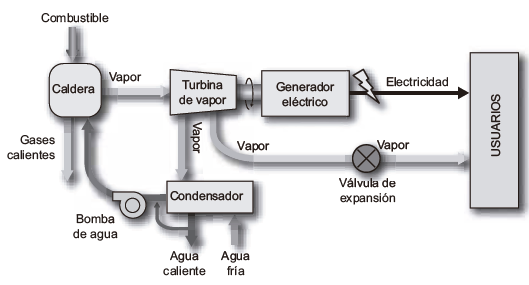
\includegraphics[width=\linewidth]{img/turbina de vapor condensacion.png} % Agregar la imagen correspondiente
    \end{columns}
\end{frame}


\begin{frame}{Turbina de gas de cogeneraci\'on}
    \textbf{Descripci\'on:}
    \begin{itemize}
        \item En este sistema, los gases calientes que salen de la turbina de gas se emplean para producir vapor.
        \item Este vapor generado puede ser utilizado para diferentes aplicaciones industriales o generaci\'on de electricidad.
    \end{itemize}
    
    \begin{minipage}{0.5\textwidth}
        \textbf{Componentes:}
        \begin{itemize}
            \item Compresor
            \item Quemador
            \item Turbina de gas
            \item Generador el\'ectrico
            \item Intercambiador de calor
        \end{itemize}
    \end{minipage}%
    \begin{minipage}{0.5\textwidth}
        \centering
        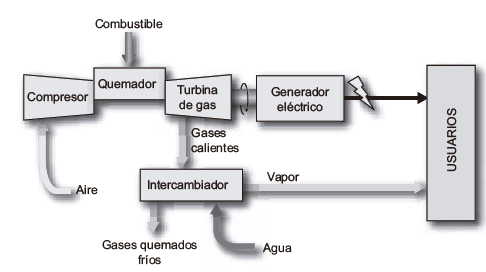
\includegraphics[width=0.9\linewidth]{img/turbinas de gas de cogeneracion.png} % Agregar imagen si se dispone
    \end{minipage}

\end{frame}
% Diapositiva: Central de cogeneración y ciclo combinado


\begin{frame}{Central de Cogeneraci\'on y Ciclo Combinado}
    \begin{columns}
        \column{0.5\textwidth}
        \begin{itemize}
            \item Combina una turbina de gas y otra de vapor en serie.
            \item Los gases calientes de la turbina de gas evaporan el agua.
            \item El vapor producido se inyecta en una turbina de vapor de condensaci\'on.
            \item Si puede usarse tambi\'en el agua caliente, el rendimiento de la transformaci\'on es m\'aximo.
        \end{itemize}
        
        \column{0.5\textwidth}
        \begin{center}
            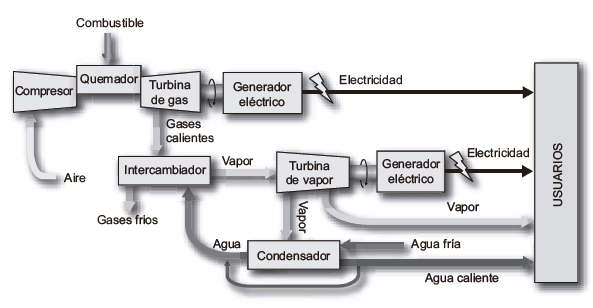
\includegraphics[width=\linewidth]{img/cogeneracion y ciclo combinado.png} % Agregar imagen si se dispone
        \end{center}
    \end{columns}
\end{frame}


%%%%%%%%%%%%%%%%%%%%%%%%%%%%%%%%%%%%%%%%%%%%%%%%%%%%%%%%%%%%%%%%%%%%

\begin{frame}{El Carbono y la Vida}
  \begin{itemize}
    \item La vida en la Tierra se basa en compuestos orgánicos formados por carbono.
    \item El CO$_2$ atmosférico y disuelto en los océanos regula los ciclos biogeoquímicos.
    \item Las plantas, mediante la fotosíntesis, son el primer eslabón de la cadena trófica.
  \end{itemize}
\end{frame}


\begin{frame}{Fotosíntesis}
  \begin{itemize}
    \item Proceso mediante el cual las plantas convierten CO$_2$ y H$_2$O en glucosa (C$_6$H$_{12}$O$_6$) y O$_2$ usando luz solar.
    \item Se realiza en los cloroplastos de las hojas verdes.
    \item Energía absorbida: aproximadamente 112 kcal/mol.
  \end{itemize}
  \begin{center}
    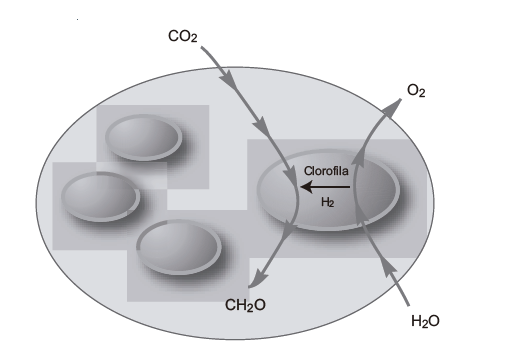
\includegraphics[width=0.5\textwidth]{img/fotosintesis.png}
  \end{center}
\end{frame}


\begin{frame}{Interacción de la Luz con la Materia}
  \begin{itemize}
    \item La energía de un fotón depende de su frecuencia: \( E = h \cdot \nu \).
    \item La luz puede:
    \begin{enumerate}
      \item Ser absorbida y disiparse como calor.
      \item Emitirse como fluorescencia o fosforescencia.
      \item Activar reacciones químicas (fotoquímica).
    \end{enumerate}
  \end{itemize}
\end{frame}

\begin{frame}{Energía en los Enlaces Moleculares}
  \begin{itemize}
    \item Un mol contiene \( 6.022 \times 10^{23} \) moléculas (constante de Avogadro).
    \item Energía promedio para romper enlaces:
    \begin{itemize}
      \item Enlace simple C–C: 82.6 kcal/mol.
      \item Enlace doble C=C: 145.8 kcal/mol.
      \item Enlace triple C$\equiv$C: 199.6 kcal/mol.
    \end{itemize}
  \end{itemize}
\end{frame}


\begin{frame}{Efectos de Diferentes Longitudes de Onda}
  \begin{itemize}
    \item Luz azul (450 nm): 64 kcal/mol.
    \item Luz infrarroja (900 nm): 32 kcal/mol.
    \item Luz ultravioleta (225 nm): 128 kcal/mol.
    \item La radiación UV puede romper enlaces químicos; la luz visible e IR no tienen suficiente energía para hacerlo.
  \end{itemize}
\end{frame}

\begin{frame}{Importancia de la Fotosíntesis}
  \begin{itemize}
    \item Es el proceso clave para la vida en la Tierra.
    \item Permite la formación de estructuras biológicas complejas y ordenadas.
    \item Origina la cadena alimentaria y mantiene el equilibrio atmosférico.
  \end{itemize}
  \[
  \text{Luz} + \text{CO}_2 + \text{H}_2\text{O} \rightarrow \text{Glucosa} + \text{O}_2
  \]
\end{frame}

\begin{frame}{Protección de los Sistemas Vivos}
  \begin{itemize}
    \item La atmósfera primitiva contenía CO$_2$ y permitía el paso de radiación UV.
    \item La fotosíntesis produjo O$_2$, que permitió la formación de ozono (O$_3$).
    \item El ozono absorbió la radiación ultravioleta, protegiendo el desarrollo de la vida.
  \end{itemize}
\end{frame}


\begin{frame}{El CO$_2$ y la Fotosíntesis}
  \begin{itemize}
    \item La fotosíntesis reduce la concentración atmosférica de CO$_2$.
    \item El CO$_2$ actual (2025): aproximadamente 420 ppm.
    \item Es esencial para el ciclo del carbono y el equilibrio climático global.
  \end{itemize}
\end{frame}

\begin{frame}{Absorción de Radiación por el CO$_2$}
  \begin{itemize}
    \item El CO$_2$ no absorbe luz visible, pero sí radiación infrarroja.
    \item La Tierra emite calor en forma de radiación IR, que es parcialmente retenida.
    \item Este efecto mantiene la temperatura media global compatible con la vida.
  \end{itemize}
\end{frame}

\begin{frame}{Papel de las Nubes y el Vapor de Agua}
  \begin{itemize}
    \item Ambos absorben y reemiten radiación IR, contribuyendo al efecto invernadero.
    \item Las nubes funcionan como aislantes térmicos.
    \item La “ventana atmosférica” permite el paso de luz visible, pero filtra UV e IR.
  \end{itemize}
\end{frame}

\begin{frame}{Radiación Solar y Clima}
  \begin{itemize}
    \item La energía solar incidente varía con la latitud y las condiciones atmosféricas.
    \item Promedios diarios (2025):
    \begin{itemize}
      \item Desiertos: 220 kcal/m$^2$/día.
      \item Zonas polares: 70 kcal/m$^2$/día.
      \item Junglas tropicales: 120–160 kcal/m$^2$/día.
    \end{itemize}
  \end{itemize}
\end{frame}

\begin{frame}{Interacción del Suelo con la Radiación}
  \begin{itemize}
    \item De día: el suelo calienta el aire por convección.
    \item De noche: el suelo pierde calor por radiación.
    \item La evaporación del agua modera el calentamiento.
    \item Suelos secos se calientan más y generan vientos térmicos.
    \item Suelos húmedos favorecen microclimas más estables.
  \end{itemize}
\end{frame}



\section{El \texorpdfstring{CO$_2$}{CO2} en la Atmósfera y el Efecto Invernadero}
\title{El CO$_2$ en la Atmósfera y el Efecto Invernadero}
\begin{frame}{Protección de los Sistemas Vivos}
    \begin{itemize}
        \item Los seres vivos necesitan protección contra la radiación ultravioleta.
        \item La atmósfera primitiva era rica en CO$_2$ y transparente a la radiación UV.
        \item La fotosíntesis liberó O$_2$, que permitió la formación de ozono (O$_3$).
        \item El ozono absorbió la radiación UV, protegiendo la vida en la Tierra.
    \end{itemize}
\end{frame}

\begin{frame}{El CO$_2$ y la Fotosíntesis}
    \begin{itemize}
        \item La fotosíntesis convirtió CO$_2$ en materia orgánica, reduciendo su concentración.
        \item Actualmente, la atmósfera contiene un 0.032\% de CO$_2$ (320 ppm).
        \item El CO$_2$ es esencial para la fotosíntesis: se convierte en hidratos de carbono mediante la energía solar.
    \end{itemize}
\end{frame}

\begin{frame}{Absorción de Radiación por el CO$_2$}
    \begin{itemize}
        \item El CO$_2$ es transparente a la luz visible, pero absorbe radiación infrarroja.
        \item La Tierra irradia calor en forma de radiación infrarroja.
        \item El CO$_2$ captura parte de esta energía y la redirige hacia la superficie.
        \item Este proceso mantiene la temperatura nocturna del suelo y la atmósfera.
    \end{itemize}
\end{frame}

\begin{frame}{El Papel de las Nubes y el Vapor de Agua}
    \begin{itemize}
        \item Las nubes y el vapor de agua también absorben y emiten radiación infrarroja.
        \item Cuando el cielo está cubierto, las nubes actúan como un manto térmico.
        \item La "ventana atmosférica" permite el paso de la luz visible, pero bloquea radiaciones UV e IR.
    \end{itemize}
\end{frame}

\begin{frame}{Radiación Solar y el Clima}
    \begin{itemize}
        \item La energía solar recibida por la Tierra varía según la región.
        \item En desiertos: 220 kcal/m$^2$/día.
        \item En zonas polares: 70 kcal/m$^2$/día.
        \item En junglas tropicales: 120-160 kcal/m$^2$/día.
    \end{itemize}
\end{frame}

\begin{frame}{Interacción del Suelo con la Radiación}
    \begin{itemize}
        \item Durante el día, el suelo transfiere calor al aire por convección.
        \item Durante la noche, el suelo pierde calor.
        \item La evaporación del agua consume energía, reduciendo el calentamiento.
        \item En suelos secos, la energía calienta la superficie y crea vientos.
        \item En suelos húmedos, la evaporación enfría el ambiente.
    \end{itemize}
\end{frame}

\begin{frame}{Conclusión: El Efecto Invernadero}
    \begin{itemize}
        \item Los gases de efecto invernadero mantienen la temperatura del planeta.
        \item Son esenciales para el equilibrio del ecosistema.
        \item Cambios en su composición pueden alterar este equilibrio y modificar los ecosistemas.
    \end{itemize}
    \begin{figure}
        \centering
        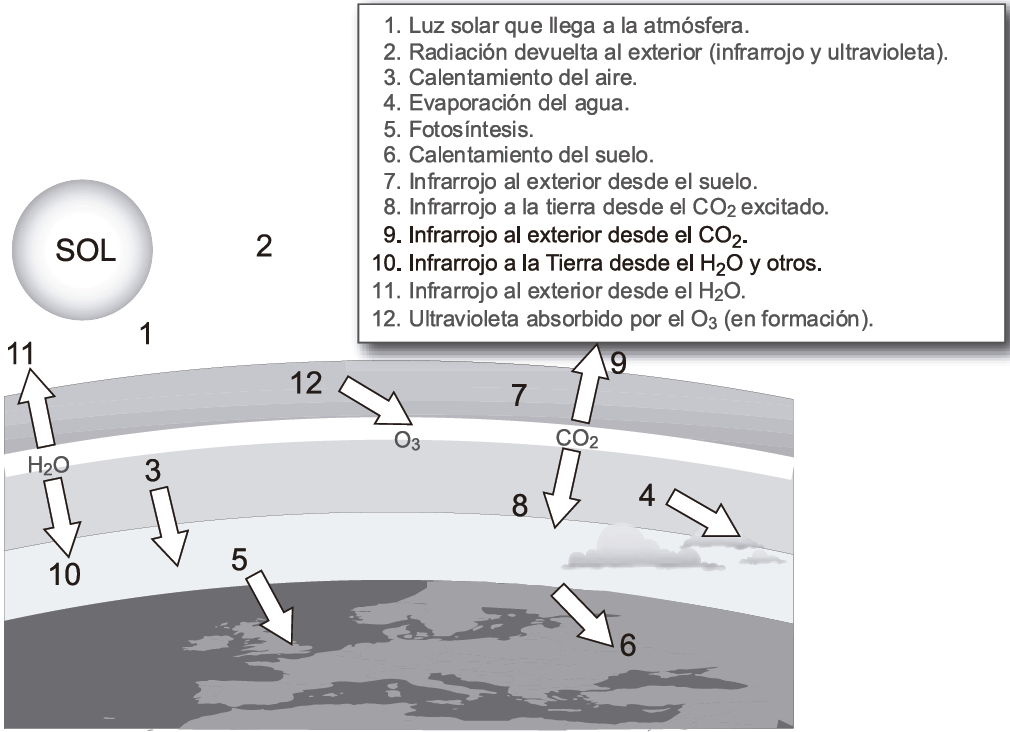
\includegraphics[width=0.5\linewidth]{img/efecto_invernadero.png}
      %  \caption{Enter Caption}
        %\label{fig:enter-label}
    \end{figure}
\end{frame}

\section{El \texorpdfstring{CO$_2$}{CO2} en el mar y el reciclado del carbono}
\title{El CO$_2$ en el mar y el reciclado del carbono}
\begin{frame}{El CO$_2$ en el mar}
    \begin{itemize}
        \item El mar actúa como un potente regulador del CO$_2$ en la atmósfera.
        \item Absorbe CO$_2$ en su superficie, especialmente por la agitación del agua.
        \item La concentración de CO$_2$ en los primeros 75 metros de agua es similar a la de la atmósfera.
    \end{itemize}
\end{frame}

\begin{frame}{Reciclado del carbono en el mar}
    \begin{itemize}
        \item Los organismos marinos contienen carbono en forma de bicarbonatos disueltos.
        \item Al morir, sus esqueletos se hunden y forman depósitos de caliza y dolomías.
        \item Estos depósitos representan el 80\% del carbono en los océanos.
    \end{itemize}
\end{frame}

\begin{frame}{Efectos a largo plazo}
    \begin{itemize}
        \item En condiciones extremas, el mar podría absorber todo el CO$_2$ en 10,000 años.
        \item Esto detendría la fotosíntesis y la actividad vital.
        \item Un exceso de absorción podría desencadenar una edad glacial.
    \end{itemize}
\end{frame}

\begin{frame}{Interacción con el ciclo del carbono}
    \begin{itemize}
        \item La actividad biológica marina regula la absorción de CO$_2$.
        \item La tectónica de placas influye en la liberación de CO$_2$ por los volcanes.
        \item El CO$_2$ de la lluvia reacciona con minerales y es transportado al océano.
    \end{itemize}
\end{frame}

\begin{frame}{Ciclo del carbono y temperatura terrestre}
    \begin{itemize}
        \item A mayor temperatura, más evaporación y lluvia, lo que extrae más CO$_2$ de la atmósfera.
        \item A menor temperatura, menos lluvia y menos extracción de CO$_2$.
        \item El ciclo del carbono mantiene la temperatura terrestre en niveles tolerables.
    \end{itemize}
    \begin{figure}
        \centering
        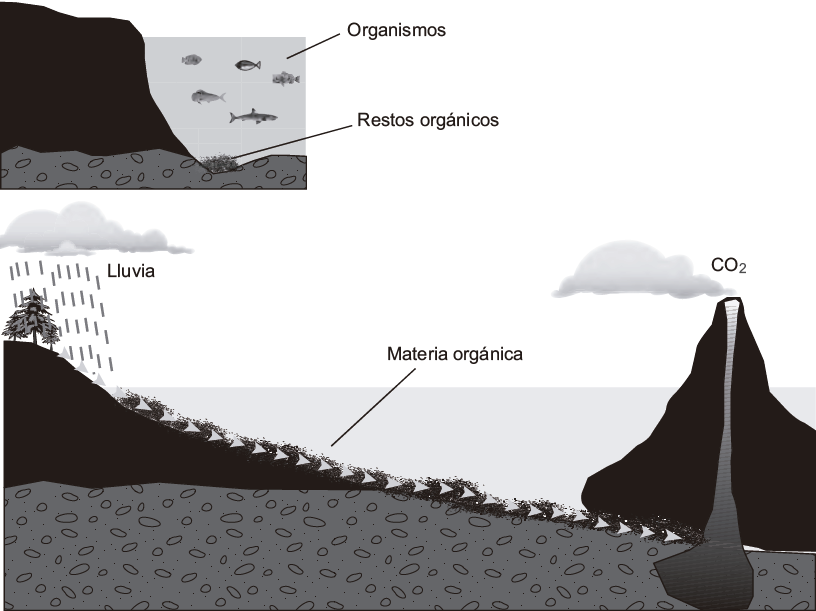
\includegraphics[width=0.5\linewidth]{img/ciclo_carbono_mar.png}
        \caption{Enter Caption}
        %\label{fig:enter-label}
    \end{figure}
\end{frame}

\section{Impacto de la Explotación de Energía en las Personas}
\begin{frame}
    \frametitle{Impacto de la Explotación de Energía en las Personas}
    La explotación de fuentes de energía tiene repercusiones sobre las personas, ya sea directamente o a través del impacto en la biosfera y el medioambiente.
    \begin{itemize}
        \item Estos efectos son mayormente negativos.
        \item Diferentes fuentes de energía tienen impactos variados.
        \item Las energías renovables tienen efectos leves.
        \item Los combustibles fósiles y la energía nuclear tienen efectos severos y duraderos.
    \end{itemize}
\end{frame}

\begin{frame}
    \frametitle{Efectos sobre la Salud Humana}
    \begin{itemize}
        \item De corto alcance: aparición de diversas enfermedades.
        \item De largo alcance: desarrollo de cáncer y otras afecciones.
        \item Impactos intergeneracionales: daños genéticos en futuras generaciones.
    \end{itemize}
\end{frame}

\begin{frame}
    \frametitle{Efectos sobre la Calidad de Vida}
    \begin{itemize}
        \item Pérdida de calidad debido a contaminación por humos y suciedad.
        \item Problemas psicosomáticos derivados del impacto ambiental.
    \end{itemize}
\end{frame}

\begin{frame}
    \frametitle{Impacto en el Empleo y Distribución Poblacional}
    \begin{itemize}
        \item Destrucción de empleos en sectores como la agricultura.
        \item Movimientos migratorios causados por inundaciones y sequías.
    \end{itemize}
\end{frame}

\begin{frame}
    \frametitle{Consecuencias para las Generaciones Futuras}
    \begin{itemize}
        \item Agotamiento de recursos naturales.
        \item Pérdida de biodiversidad y deterioro de ecosistemas.
    \end{itemize}
\end{frame}







\section{Cambio Climático}

\begin{frame}{Cambio Climático}
    \begin{itemize}
        \item La combustión de combustibles fósiles ha incrementado la concentración de CO$_2$ en la atmósfera, pasando de 280 ppm en la era preindustrial a más de 415 ppm en la actualidad.
        \item Se estima un aumento de temperatura de 2-4.5$^{\circ}$C para el año 2050 si no se reducen las emisiones.
        \item Consecuencias:
        \begin{itemize}
            \item Pérdida de glaciares y aumento del nivel del mar, afectando a comunidades costeras.
            \item Cambios climáticos extremos como huracanes más intensos, olas de calor y sequías prolongadas.
            \item Reducción de la producción agrícola y riesgo de inseguridad alimentaria.
            \item Impacto en la biodiversidad con la extinción de especies sensibles al cambio climático.
        \end{itemize}
    \end{itemize}
\end{frame}

\section{Lluvia Ácida}

\begin{frame}{Lluvia Ácida}
    \begin{itemize}
        \item Derivada de la combustión de carbón y petróleo, ricos en azufre y nitrógeno, que generan dióxido de azufre (SO$_2$) y óxidos de nitrógeno (NO$_x$).
        \item Estos contaminantes reaccionan con el agua en la atmósfera formando ácido sulfúrico y ácido nítrico.
        \item Consecuencias:
        \begin{itemize}
            \item Acidificación del suelo, afectando la absorción de nutrientes por las plantas.
            \item Destrucción de bosques, especialmente en regiones montañosas con ecosistemas frágiles.
            \item Daño a ecosistemas acuáticos por la alteración del pH del agua.
            \item Corrosión de infraestructuras, monumentos históricos y edificaciones.
        \end{itemize}
    \end{itemize}
\end{frame}

\section{Destrucción de la Capa de Ozono}

\begin{frame}{Destrucción de la Capa de Ozono}
    \begin{itemize}
        \item Causada principalmente por compuestos químicos como los clorofluorocarbonos (CFCs) y los óxidos de nitrógeno.
        \item Estos compuestos destruyen el ozono (O$_3$) en la estratósfera, reduciendo la protección contra la radiación ultravioleta (UV).
        \item Consecuencias:
        \begin{itemize}
            \item Aumento de enfermedades como cáncer de piel y cataratas.
            \item Disminución de la productividad agrícola por daño en cultivos sensibles a la radiación UV.
            \item Alteración de ecosistemas marinos, afectando el fitoplancton, base de la cadena alimenticia oceánica.
        \end{itemize}
    \end{itemize}
\end{frame}

\section{Impacto en Suelo y Aguas}

\begin{frame}{Impacto en Suelo y Aguas}
    \begin{itemize}
        \item Contaminación del suelo por la extracción y refinamiento de combustibles fósiles, afectando la biodiversidad y la calidad del suelo.
        \item Derrames de petróleo que contaminan mares y océanos, causando daños irreparables a la fauna marina.
        \item Filtración de metales pesados y sustancias tóxicas en aguas subterráneas, afectando el agua potable.
        \item Efectos de la lluvia ácida en ríos y lagos, alterando la composición química del agua y perjudicando la vida acuática.
    \end{itemize}
\end{frame}

\section{Impacto de las Energías Renovables}

\begin{frame}{Impacto de las Energías Renovables}
    \begin{itemize}
        \item Mínimo impacto ambiental en comparación con las energías fósiles, al no generar emisiones de gases de efecto invernadero.
        \item Energía hidráulica puede generar impacto ambiental por la construcción de presas, que alteran los ecosistemas fluviales.
        \item Energía eólica y solar han reducido costos y mejorado su eficiencia, promoviendo su uso masivo.
        \item Desarrollo de tecnologías de almacenamiento, como baterías de litio y sistemas de hidrógeno verde, para garantizar estabilidad en la generación de energía.
    \end{itemize}
\end{frame}

\section{Protocolo de Kioto y Acuerdo de París}

\begin{frame}{Protocolo de Kioto y Acuerdo de París}
    \begin{itemize}
        \item El Protocolo de Kioto (1997) fue el primer acuerdo internacional para reducir las emisiones de gases de efecto invernadero, estableciendo compromisos para los países desarrollados.
        \item Mecanismos de flexibilización:
        \begin{itemize}
            \item Comercio de Derechos de Emisión: los países pueden comprar y vender cuotas de emisión de carbono.
            \item Implementación Conjunta: permite a los países desarrollados financiar proyectos de reducción de emisiones en otras naciones.
            \item Mecanismo de Desarrollo Limpio: fomenta proyectos sostenibles en países en desarrollo.
        \end{itemize}
        \item El Acuerdo de París (2015) reemplazó a Kioto, con compromisos de reducción de emisiones para todos los países, con el objetivo de limitar el calentamiento global a menos de 2$^{\circ}$C.
        \item Promueve la inversión en energías renovables y la adaptación al cambio climático.
    \end{itemize}
\end{frame}


\section{Los Costes de la Energía}
\title{Los Costes de la Energía}

\begin{frame}{Introducción Los Costes de la Energía}
\begin{itemize}
    \item \textbf{Coste} es la cantidad a la que ha de venderse una unidad de energía (1 kWh) al usuario final para que se obtenga una rentabilidad aceptable (prevista) de la inversión (en equipos, redes de distribución, explotación, etc.).
    \item \textbf{Precio} es la cantidad que en cada instante el mercado paga por 1 kWh de energía (o la
cantidad a la que se compra el kWh).
\end{itemize}


    \begin{itemize}
        \item Diferencia entre coste y precio de la energía.
        \item Expresión del coste en \$/kWh o \$/kW instalado.
        \item Consideración de costes internos y externos.
        \item Clasificación en costes fijos y variables.
    \end{itemize}
\end{frame}


\begin{frame}{Los Costes Internos}
    \begin{itemize}
        \item Costes de capital:
        \begin{itemize}
            \item Preparación e ingeniería.
            \item Construcción e integración.
            \item Gestión del proyecto y seguros.
        \end{itemize}
        \item Costes circulantes:
        \begin{itemize}
            \item Operación (combustible, personal, seguros).
            \item Mantenimiento (revisiones, reparaciones).
        \end{itemize}
        \item Otros costes:
        \begin{itemize}
            \item Overheads y costes de finalización.
        \end{itemize}
    \end{itemize}
\end{frame}

\begin{frame}{Costes de la Energía y Precio del Dinero}
    \begin{itemize}
        \item Influencia de la inflación y el interés en el coste de la energía.
        \item Cálculo del coste del kWh considerando capital y costes circulantes.
        \item Dependencia del coste con la producción energética.
    \end{itemize}
    En definitiva, y de acuerdo con esta variable, el coste de la energía (kWh) se calcula así:
\begin{itemize}
    \item Se dividen los costes de capital por el número de años en funcionamiento, y se calcula el valor presente para el año 0 (considerando inflación, intereses, etc.).
    \item Se calcula el valor medio de los costes circulantes, y se actualizan para el año 0.
    \item Se suman las dos cantidades anteriores y se dividen por el número de kWh que la máquina, central, etc. produce.
\end{itemize}

Se observa que el coste depende de la producción. En el caso de energías renovables, la correcta previsión de ésta es esencial para determinar su coste.
\end{frame}

\begin{frame}{Costes de la Energía y Recursos Disponibles}
    \begin{itemize}
        \item Relación entre el coste y la cantidad de recurso disponible.
        \item Incremento del coste con el agotamiento de recursos accesibles.
    \end{itemize}
    \begin{figure}
        \centering
        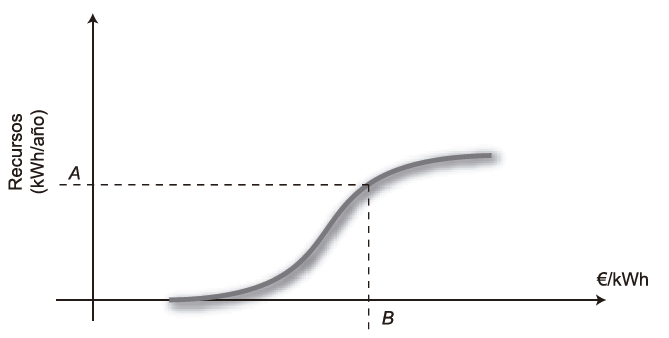
\includegraphics[width=0.5\linewidth]{img/costos_Vs_disponibilidad.png}
        \caption{Variación del coste en función de la disponibilidad del recurso.}
        %\label{fig:enter-label}
    \end{figure}
\end{frame}


\begin{frame}{Los Costes Externos}
    \begin{itemize}
        \item Costes de salud: enfermedades leves y graves.
        \item Costes medioambientales: daños en flora, fauna y cambio climático.
        \item Costes a largo plazo por agotamiento del recurso.
        \item Costes de seguridad y conflictos geopolíticos.
    \end{itemize}
\end{frame}


\begin{frame}{Impacto sobre Energías Renovables}
    \begin{itemize}
        \item No inclusión de costes externos distorsiona el precio real de la energía.
        \item Energías renovables frenadas por precios bajos de fósiles y nucleares.
        \item Beneficios sociales podrían equilibrar costes con energía convencional.
        \item Falta de incentivos para el ahorro y eficiencia energética.
    \end{itemize}
\end{frame}

\begin{frame}{Conclusión}
    \begin{itemize}
        \item Necesidad de considerar todos los costes (internos y externos).
        \item Incorporación de externalidades para una comparación justa.
        \item Posible transición hacia energías renovables con políticas adecuadas.
    \end{itemize}
\end{frame}



\end{document}